\documentclass[11pt]{report}
\bibliographystyle{ieeetr}
\usepackage[a4paper, total={6in, 8in}]{geometry}
\usepackage{amsmath}
\usepackage{blindtext}
\usepackage{parskip}
\usepackage{enumitem}
\usepackage[nottoc,numbib]{tocbibind}
\usepackage[section]{placeins}
\usepackage{graphicx} % Required for inserting images
\usepackage[english]{babel}
\usepackage{pdfpages}
\usepackage{xargs}                      % Use more than one optional parameter in a new commands
%\usepackage[pdftex,dvipsnames]{xcolor}  % Coloured text etc.
%
\usepackage[colorinlistoftodos,prependcaption,textsize=tiny]{todonotes}
\newcommandx{\unsure}[2][1=]{\todo[linecolor=red,backgroundcolor=red!25,bordercolor=red,#1]{#2}}
\newcommandx{\change}[2][1=]{\todo[linecolor=blue,backgroundcolor=blue!25,bordercolor=blue,#1]{#2}}
\newcommandx{\info}[2][1=]{\todo[linecolor=OliveGreen,backgroundcolor=OliveGreen!25,bordercolor=OliveGreen,#1]{#2}}
\newcommandx{\improvement}[2][1=]{\todo[linecolor=orange,backgroundcolor=orange!25,bordercolor=orange,#1]{#2}}
\newcommandx{\thiswillnotshow}[2][1=]{\todo[disable,#1]{#2}}

\usepackage{acro}
\usepackage[colorlinks=false]{hyperref}
\usepackage{pdfcomment}

\acsetup{
	make-links 		= 	false,
	pdfcomments/use		=	true,
}

\DeclareAcronym{VTC}{short = {VTC}, long = {Value-transfer chain}, pdfcomment = {Value-transfer chain}}

\DeclareAcronym{GPC}{short = {GPC}, long = {General-purpose chain}, pdfcomment = {General-purpose chain}}
%\DeclareAcronym{ESG}{short = {ESG}, long = {Environmental Social \& Governance}, pdfcomment = {Environmental Social \& Governance}}
\DeclareAcronym{CCRI}{short={CCRI}, long={Crypto Carbon Ratings Institute}, pdfcomment = {Crypto Carbon Ratings Institute}}


\parskip 2ex
\parindent 0pt

\title{GreenBlocks - SMT PdM}
\author{mbelanger.poly}
\date{August 2023}


\begin{document}

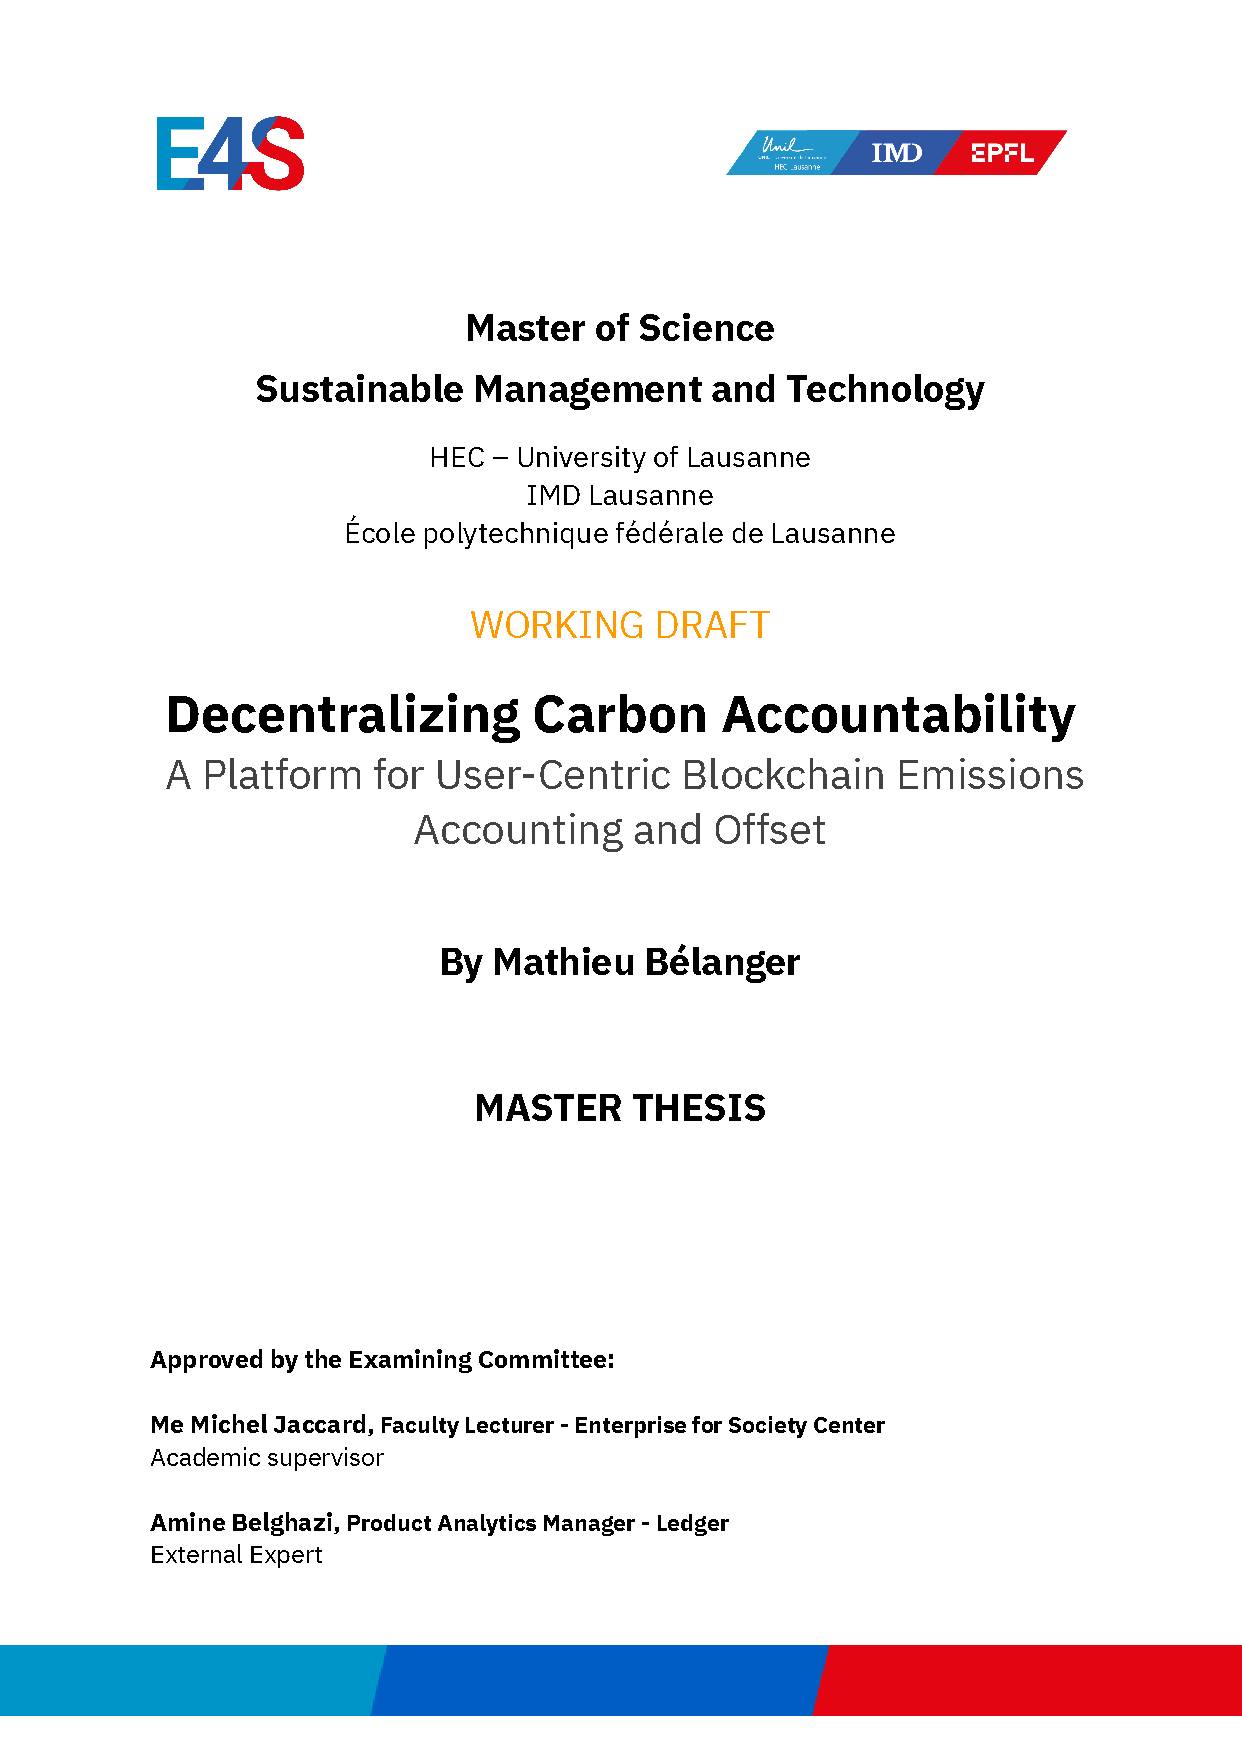
\includepdf[pages={1-2}]{cover.pdf}
\section*{Abstract}
\change{Put abstract in e4s template}
\improvement{Too long}

Executive summary.
The advent of blockchain technology has raised concerns about its high energy use and carbon emissions. This is partly due to the current dominance of proof-of-work-driven Bitcoin, the first network to gain widespread adoption and media coverage. A growing research corpus has established and compared the varying environmental footprints across blockchains, resulting from different consensus mechanisms and design choices. While the recent release of the first industry blockchain ESG benchmark enables standardized comparisons between chains at an aggregate level, granular methodologies for user-level emissions accounting are still in their infancy. This thesis objective is to compare emissions attribution approaches in order to develop à proof-of-concept tool for user-level on-chain accounting and offsetting.

Building upon state-of-the-art emissions acconuting research this thesis revises attribution models designed to map the carbon footprint of blockchain at a user-responsibility level. Novel to this research, is the attempt to weigh responsibility factors based on the principle of proportional benefit (hybrid attribution). This approach exploits the inherent transparency of blockchain data to capture the relative value, specific to each network, that users place on different blockchain functionalities. Consistent to prior reseach, we find that two generalizable categories of benefits emerge: the Transactional use case (benefits from active transacting or interacting) and the Asset-Securing use case (benefits from passively holding or securing assets). Key parameters such as asset balance, signed transactions, and gas expenditure are used as representative indicators of benefiting from a network use case. This methodology allocates the overall chain emissions to specific users based on their interaction patterns. The evolutions of network-specific transaction fees and market capitalization are used to derive weight for these parameters. All in all, it is established that hybrid allocation methods are not sufficiently accurate to be used as a standalone attribution model. However, they can be used as a complementary approach to existing methodologies, providing a more nuanced perspective on the relative responsibility of users.

Furthermore, a proof-of-concept tool (GreenBlocks) is built to showcase the attribution models, allowing users to estimate and offset their emissions through carbon credits. Based on the Ledger Live platform, this platform interacts seamlessly with leading blockchains and links with on-chain carbon market partners to retire offsets with maximal transparency.

Greenblocks provides transparent and personalized insights into blockchain emissions for end-users. By linking usage to quantified environmental impact, it promotes awareness. It enables offsets as a means for users to bear the actual costs behind the benefits they reap from using the technology. Moreover, it demonstrates the potential for on-chain data to be used as the foundation for an appropriately nuanced attribution of external costs in a system. Moving past rudimentary address metrics, more complex behaviors and benefits can be modeled, potentially  enabling the distribution of externalities like a Pigouvian tax. Thus, this thesis proposes a bottom-up, user-focused approach to align blockchain adoption with environmental sustainability. This is achieved by pioneering user-level footprint attribution, arising from the \textit{Benefiiciary pays principle}.


\change{Add section on further opportunities for the blockchain-sustainability space}

\newpage
\section*{Acknowledgements}
\tableofcontents



\chapter{Introduction}

\section{Background and Motivation}
\improvement{Compartiment in subsections to improve narrative flow}
\subsubsection*{Origins, promise and challenges of blockchain technology}
The advent of blockchain technology since the launch of Bitcoin in 2009 has sparked a revolution in systems of value transfer, transparency, and decentralization \cite{nakamotoBitcoinPeertopeerElectronic2008}. However, the early meteoric rise of cryptocurrencies and underlying blockchain networks has raised critical concerns regarding their environmental sustainability. With the benefit of hindsight, we can view this period as Gartner's Peak of Inflated Expectations. Now, with notorious founders imprisoned, increasing regulatory scrutiny, and the total cryptocurrency market capitalization down
XX\% from its peak \change{cite}, the blockchain ecosystem stands at a crossroads. This is an opportunity to refocus on the core propositions of blockchain technology and ensure its long-term viability.


The dominant network, Bitcoin, which utilizes a computationally-intensive proof-of-work consensus mechanism, has attracted particular scrutiny for its high energy consumption. Recent estimates indicate the Bitcoin network alone may consume between 115 and 150 TWh annually, comparable to entire countries like the Netherlands \cite{devriesRevisitingBitcoinCarbon2022,neumuellerCambridgeBitcoinElectricity2021}. This growing apetite for energy competes with the just starting energy transition, putting electrical production and distribution networks under stress. Finally it also results in significant CO2 emissions, hardly compatible with global climate goals like the Paris Climate Accords.

\subsubsection*{Limitations of current approaches}
However, we must recognize the complexity and nuance when evaluating blockchain sustainability. Consensus protocols, design choices, and use cases vary greatly across different networks, leading to wide variability in energy needs and emissions. For instance, proof-of-stake networks like Cardano and Solana promise energy savings by factors of 1000x or more compared to proof-of-work \cite{kohliAnalysisEnergyConsumption2023}. Moreover, Ethereum recently completed its highly anticipated, technically and politically complex transition from proof-of-work to proof-of-stake, demonstrating that such migrations are viable for major networks. \cite{bloombergnewsEthereumMergeYour2022} The nascent field of blockchain sustainability analysis must evolve more granular, differentiated perspectives.

Initial responses from the blockchain industry have focused on high-level aggregate comparisons and rankings between networks. For example, recent benchmarks like the \ac{CCRI} methodology provide standardized comparisons of the total lifecycle emissions across chains [5]. In parallel to this work the institute partnered with researchers in order to further develop attribution methodologies, this will be disucssed in the \textit{Previous Work section} \ref{ch:previous_work}. The CCRI However, these overlook the diversity of users and fail to provide accountability at an individual level.
\todo{include CCRI work on emissions accounting}

This poses a critical gap, especially as blockchain technology expands into mainstream adoption. We lack a methodology to attribute network-wide emissions to specific users based on their unique activity patterns and values. Such granular carbon accounting can raise awareness of individual impact and empower ethical participation.

\subsubsection*{Opportunities for user-level footprinting}

To address this, the novel approach in this thesis involves an attribution model that weighs factors like asset holdings, transactions, and computations based on their estimated importance to users on each chain. By considering relative user perspectives, we can map emissions more accurately to individual entities like protocols, DAOs, or end-users. This unconventional yet powerful approach unlocks new potentials for transparency, responsibility, and sustainability.

\begin{figure}[hbt!]
    \centering
    \centerline{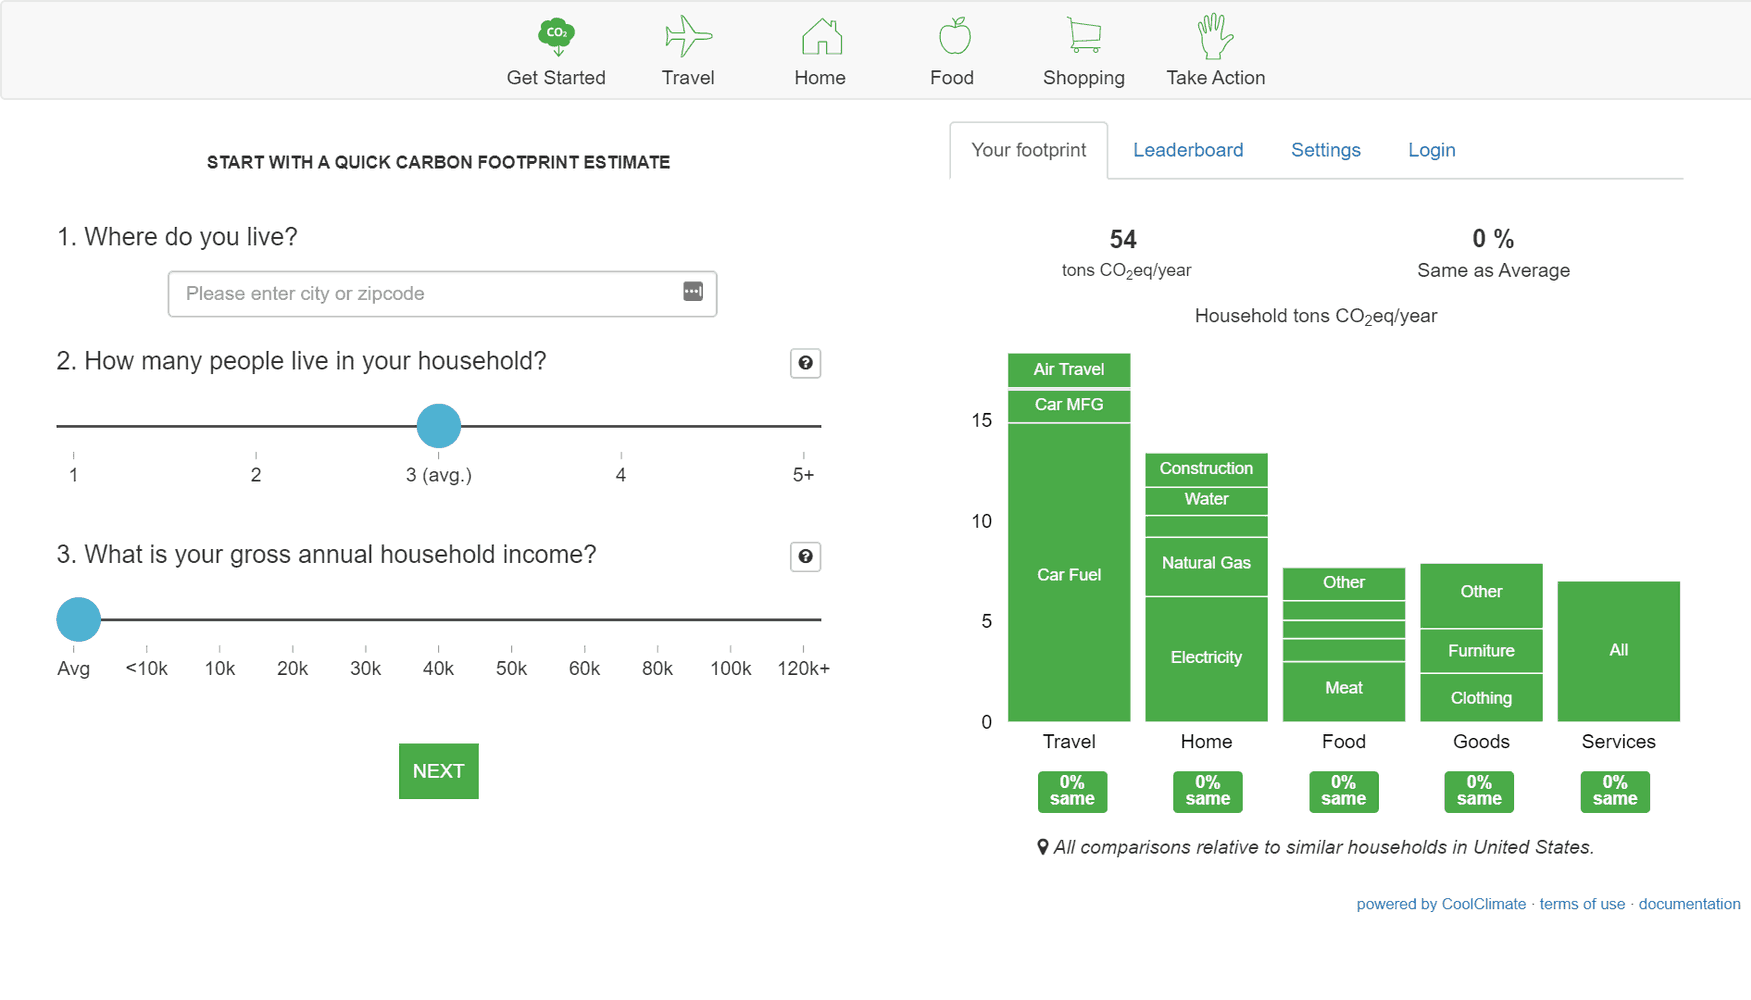
\includegraphics[scale=0.25]{figures/carbon_footprint_calculator.png}}
    \caption[YO]{Tradionnal carbon footprint calculator form - CoolClimate\footnotemark}
    \label{fig:carbon_footprint_calculator}
\end{figure}

\footnotetext{https://coolclimate.org/calculator}

Limited User engagement towards footprint calculators, tedious process and error prone \cite{saloOpportunitiesLimitationsCarbon2019,mulrowStateCarbonFootprint2019}.

\todo{This is the user experience that will be improved with blockchain data transparency and attribution. Link wiht further use sustainability use cases. Blockchain based footprints makes possible automating the process and vastly increases accuracy as it is no more a self assesment. Cite issues of carbon footprint calculator accuracy because of self assesment.}
\section{Problem Statement}

As blockchain technology progresses into mainstream integration, the lack of transparency and accountability for emissions at an individual user level poses a critical gap. For example, retail investors drawn to crypto assets may be unaware of the passive environmental impacts associated with their portfolios over time. There is also increasing offering of decentralized applications (web3) with usage beyond those of investing. Granular carbon accounting and attribution to individual wallets can raise awareness and enable offsetting as a means for users to take responsibility of their actions.

Moreover, this gap becomes even more complex for providers of decentralized apps or decentralized autonomous organizations (DAOs) comprising multiple smart contracts and user addresses. Without a methodology for attributing network-wide emissions based on collective usage patterns, a DAO cannot fully assess and mitigate its overall carbon footprint.

Therefore, the overarching problem this thesis addresses is:

"How can we design an attribution model that allocates the carbon emissions of any blockchain network to specific user entities or addresses in a transparent, accurate, and relevant manner based on their unique activity patterns?"

\subsubsection{Carbon Offsets - The Voluntary Carbon Market}
\textbf{Traditionnal Offsets - Limitations}
\textbf{Bringing Offsets On-Chain - Opportunities }

\section{Research Questions and Ojbectives}

To systematically address the problem of transparent and accurate carbon attribution for blockchain users and entities, this thesis pursues four key research questions:

\begin{enumerate}
    \item How can blockchain emission factors be quantified at a granular, user-centric level, beyond aggregate network-wide estimates?
    \item What are appropriate metrics and weighting systems to reflect the responsibilities of diverse blockchain users based on their activities?
    \item How can we validate and demonstrate such an attribution model through a practical implementation?
    \item What are the broader implications of user-centric emissions accounting for accelerating sustainability as blockchain technology matures?
\end{enumerate}

The main objectives of this work are:

\begin{description}

    \item [Develop a User-Level Attribution Model] \hfill \\
          Develop a robust emissions attribution methodology based on usage and responsibility.
    \item [Greenblock: Pratical Application] \hfill \\
          Implement and validate the model through a functional proof-of-concept application.
    \item [Promote awareness and Responsibility] \hfill \\
          of environmental impact among blockchain users.
    \item [The Future of Sustainability and Blockchain] \change{to complete}
\end{description}

\section{Scope and Limitations}
TO COMPLETE
\todo{Focus on environmental sustainability, CO2e emissions. Not other externalities like e-waste, social impact, etc.}


\section{Structure of the Thesis}
TO COMPLETE

\chapter{Previous Work} \label{ch:previous_work}

\todo{Purpose and scope of literature review}

\section{Blockchain Technology and Its Evolution}

"Bitcoin: A Peer-to-Peer Electronic Cash System", the mysterious whitepaper \cite{nakamotoBitcoinPeertopeerElectronic2008}, published under the pseudonym Satoshi Nakamoto in 2008, was the first to propose a fully decentralized electronic cash system based on cryptographic proof instead of trust. It introduced the concept of proof-of-work mining to timestamp transactions and secure the network through computational power rather than centralized authorities. Proof-of-work was chosen to enable a distributed consensus mechanism and one-CPU-one-vote majority decision making resistant to sybil attacks. It also provides an economic incentive for miners to support the network. Overall, Bitcoin's proof-of-work system enabled the first widely adopted decentralized digital currency by solving the double-spend problem without requiring a trusted third party.\improvement{Reasons why proof-of-stake was chosen for bitcoin and why it works well. Reasons that prevented previous attempts to succeed.}

The Ethereum whitepaper\cite{buterinEthereumNextgenerationSmart}, published by Vitalik Buterin in 2013, proposed enhancements to allow decentralized applications beyond just currency. It introduced smart contracts, which are executable codes hosted on the blockchain that can encode complex logic and state. Along with a Turing-complete programming language to write smart contracts, this enabled arbitrary applications to be built on its decentralized infrastructure. Ethereum also improved upon Bitcoin's proof-of-work with proposed upgrades like GHOST and differentiated gas costs based on computation complexity. While Bitcoin demonstrated a currency application, Ethereum expanded the potential of blockchains to diverse sharing economies, financial services, identity systems and beyond. Moving past Bitcoin's singular focus, Ethereum highlighted how decentralized consensus mechanisms like blockchain could provide a foundation for customizable peer-to-peer applications. \improvement{Differences in design choices and features. Opportunities for scaling blockchains horizontally to more usecases. This is the inception of blockchain technology as an ubiquitous infrastructure.}

\cite{bloombergnewsEthereumMergeYour2022} \todo{add ethereum transition to PoS, should bitcoin do the same, why it didnt and is it likely to change}

\cite{easleyMiningMarketsEvolution2019}\todo{add analysis of bitcoin tx fees, influence on the dynamics of users participation. Gradually becoming the only incentive for miners. Thus no transaction no security.}

\section{Environmental Impact of Blockchains}
\subsection{Bitcoin and Proof-of-Work}
The environmental impact of Bitcoin, driven by its proof-of-work consensus mechanism, has become an important focus in research and public discussion. The main concern is Bitcoin's energy-intensive mining process and associated carbon emissions. As research has evolved, a nuanced understanding of Bitcoin's environmental footprint requires examining multiple factors, combining economic modeling and empirical data analysis. Estimates can adopt two different approach, top-down or bottom-up. Top-down approaches infer energy (and emissions) use from the evolving valuation of mined tokens, applying hypothesis on aggregate miners economics and behavior. Bottom-up approaches on the other hand are slightly more complex. They use empirical data on available hardware and transparent network hashrate data (the evolving mining difficulty factor specific to each chain) to work upwards to overall energy use and emissions. The following sections review the main findings from both approaches.

\textbf{Bitcoin's Energy Consumption}

De Vries (2018) \cite{devriesBitcoinGrowingEnergy2018} shed light Bitcoin mining's vast energy demands, estimating the network could consume over 73 TWh/year at peak performance, approaching entire countries' consumption. This stemmed from the immense computational power needed for mining, with energy expenditures of 300-900 kWh per transaction. De Vries' analysis used economic models, suggesting miners operate up to where electricity costs dominate marginal costs. De Vries used a top-down approach.

Stoll et al. (2019) \cite{stollCarbonFootprintBitcoin2019} refined these estimates using a techno-economic approach, still considered top-down. They diverged from De Vries in deriving hardware efficiency data from mining manufacturer IPOs and using IP geolocation for localized emission factors. Their findings showed 45.8 TWh consumption in 2018, substantial but below De Vries' projection. Incorporating IP distribution scenarios offered valuable localization insights into Bitcoin's energy sources.

\textbf{Beyond Energy: Environmental Externalities}

While energy is the primary focus, De Vries (2021) \cite{devriesBitcoinGrowingEwaste2021} highlighted another issue: e-waste. Mining hardware obsolescence contributes over 30.7 metric kilotons/year of e-waste, underscoring Bitcoin's multifaceted environmental challenges beyond energy. De Vries' lifecycle analysis methodology offered more rigorous e-waste estimates than previous energy-focused models.

\textbf{Impacts of Regulatory Shifts}


Bitcoin's dynamic landscape, influenced by regulation, also affects its environmental impact. De Vries (2022)\cite{devriesRevisitingBitcoinCarbon2022}  revisited Bitcoin's carbon footprint after China's 2021 mining crackdown. This led renewable energy's share in mining to drop from 42\% to 25\%, as miners relocated to Kazakhstan and the US. Such shifts demonstrate Bitcoin's unstable regulatory landscape and the dramatic impact it can have on environmental performance.

\textbf{Live Emission Monitoring}

The Cambridge Bitcoin Electricity Consumption Index \cite{neumuellerCambridgeBitcoinElectricity2021} and accompanying Greenhouse Emissions's Index
exemplifies cutting-edge emission monitoring, continually tracking Bitcoin's emissions using real-time, localized data and daily emission factors. This robust bottom-up approach captures the dynamics of cryptocurrency mining emissions and has been corroborated by other methodologies, including different bottom-up estimates \cite{mcdonaldEthereumEmissionsBottomup2022}.

\section{Ethereum, the Succesful Case for a Transition to Proof-of-stake}

Ethereum's recent shift from the energy-intensive "proof-of-work" consensus mechanism to the more sustainable "proof-of-stake" in september 2022 has been transformative for the cryptocurrency landscape. This transition, known as "the Merge", was long delayed due to the technical and political complexities putting in jeopary a succesful transition. Now achieved, it positions Ethereum as a leader in blockchain sustainability\footnote{https://ccdata.io/research/esg-rankings} and sets a precedent for other major cryptocurrencies to consider transition. With Ethereum's move expected to drastically reduce its carbon footprint, focus is turning to Bitcoin's potential trajectory. While the two platforms serve different primary functions, Ethereum's successful transition raises the question: Could Bitcoin be next to adopt a greener consensus mechanism?

\textbf{Ethereum's Energy Use (PoW)}

McDonald (2022)\cite{mcdonaldEthereumEmissionsBottomup2022} tackled Ethereum's energy footprint through a meticulous bottom-up approach. By compiling data on network hashrates, hardware efficiencies, and even datacenter overheads, McDonald thoroughly modeled Ethereum's consumption at ~60 TWh over seven years. Aligning with top-down estimates, this empirically-grounded, best-practice approach highlighted the need for more sustainable consensus mechanisms.

\textbf{Exploring PoS' Potential}

Exploring PoS as an energy-efficient PoW alternative has gained momentum. Platt et al. (2021)\cite{plattEnergyFootprintBlockchain2021} analyzed PoS chains' energy needs, pioneering a model weighing factors like validator counts and node power. Findings were promising: PoS chains consumed far less energy than PoW counterparts, with some even outperforming centralized systems like VisaNet.

Ibanez (2023) built on this, validating the model's core findings while highlighting nuances in consumption across PoS systems. Crucially, their research emphasized PoS systems' relative efficiency compared to heavyweights like Bitcoin.

\textbf{Ethereum's PoS Transition: A Case Study}

Ethereum's 2022 merge to PoS marked a sustainability milestone. De Vries (2022)\cite{devriesCryptocurrenciesRoadSustainability2022} thoroughly examined this transition. The anticipated post-merge energy use reduction is monumental - nearly 99.95\%, potentially equivalent to a country like New Zealand's electricity. While challenges around e-waste and wealth concentration risks remain, Ethereum's move sets a precedent, demonstrating blockchains can scale sustainably.

\section{Carbon Accounting - User-Level Emissions Attribution}

Amid rising institutional concerns about cryptocurrencies' environmental impact, the Crypto Carbon Ratings Institute's (2023)\ revised white paper provides a timely, nuanced perspective. By thoroughly examining the carbon footprints of both PoW and PoS networks, the paper introduced in its most recent version an "hybrid allocation" approach for emissions accounting. This methodology recognizes that network energy use stems from both holdings and transactions.

It expands on previous work by De Vries (2021) \cite{devriesTrueCostsDigital2021}, early attemps at an address balance emisssion attribution methdology for bitcoin. The CCRI's methodology now covers a wide range of networks, differentiating between PoS and PoW in the attribution strategy. Specifically, they use a combination of the Cambridge Index \cite{neumuellerCambridgeBitcoinElectricity2021}, de Vries "Revisiting Btcoin's carbon footprint" \cite{devriesRevisitingBitcoinCarbon2022} and Gallersdörfer's work \cite{gallersdorferEnergyConsumptionCryptocurrencies2020} for PoW chains (Bitcoin, ETH PoW in our case). For PoS networks (ETH PoS in our case) the methdology is reported in their own \textit{ETH Merge Report}\cite{ETHMergeReport}, it expands on the work of Platt et al. (2021)\cite{plattEnergyFootprintBlockchain2021} and Ibanez et al. (2023)\cite{ibanezEnergyConsumptionProofStake2023}.

\textbf{The Hybrid Allocation Approach}

The "hybrid allocation" approach is a significant contribution, merging holding-based and transaction-based emissions accounting for a comprehensive view of blockchains' environmental impact. For PoW chains, the relationship between block rewards and transaction fees is used to weight both variables in the attribution formula. According to the authors, this proportion "determines the distribution of the electricity consumption between holding and transactions executed". For PoS chains, the marginal power demand resulting from processing transactions is used as a share of total demand.\todo{Reread and check with framework version slides if it is also the case} Real-world data sources like CBECI and their owen CCRI-API back this methodology.

\subsection{Identifying a research gap}

While aligning with the CCRI's recent approach to hybrid attribution, this research introduces the "Beneficiary Pays Principle" to weigh emissions responsibility based on users' perceived value from blockchain functions. This user-centric approach provides a differentiated perspective to the paper's focus on block rewards and fees.

Moreover, the CCRI paper lacks a practical implementation of its methodology and beyond user-example results. This thesis addresses this gap by building a proof-of-concept application to demonstrate the attribution model's feasibility and value.

\subsection{Traditionnal Individual Carbon Footprint}
\subsection{Blockchain Adress Footprint}
\section{Research Gap}


\chapter{Methodology: User-Level Emissions Attribution Model}
\section{Overview}

\todo{Find where to include steps of the work. Interviews and data collection}

As blockchain technology expands onto more use cases and scale in it adoption, quantifying and attributing associated carbon emissions transparently emerges as a valid need. While aggregate estimates provide high-level network overviews, they fail to offer accountability at an individual user level, posing a user education gap and potentially a product need.

This chapter introduces a novel methodology to attribute network emissions to specific blockchain addresses based on proportional benefits gained by users. By mapping network footprints to end-users, protocols, and DAOs, this framework enables entities to understand, report, and take action based on their responsibility in the overall emissions.

The methodology is underpinned by ethical and economic theories suggesting emissions be allocated based on the proportional benefits users derive, both actively through transferring value and interacting, and passively from securing assets. Historical trends in activity metrics like fees and market value provide useful signals into evolving blockchain utility dynamics and user perceptions of value.

By incorporating these perspectives, the model aims for a fair, customizable attribution aligned with the real-world value users obtain from blockchain networks. The following sections detail this approach and rationale.

\section{Background - Emission attribution considerations}

\subsection{Blockchain Typology}
Blockchains can be categorized into two main types based on their primary function and underlying mechanics:
\improvement{this separation is also justified by the polluter and beneficiary pays framework. The limited ressource (blockspace) is shared differently for bitcoin and ethereum}

\begin{description}
    \item[\ac{VTC}] Chains that focus on transferring assets between addresses (e.g. Bitcoin and derived). VTCs are focused primarily on enabling value transfers through native cryptocurrency tokens. These chains do not typically support complex smart contract functionality like GPCs or make similar functionalities unergonomic to implement. The key operational metric for VTCs is the transaction throughput, constrained by blocksize and block intervals.

    \item[\ac{GPC}] Chains that allow the deployment of smart contracts and decentralized applications (dApps) in addition to value transfer (e.g. Ethereum, Cardano, Solana). On these networks, transactions and computations are quantified using a metric called gas\footnote{See: https://ethereum.org/en/developers/docs/gas/}. This concept was introduced by Vitalik Buterin in Ethereum's initial whitepaper \cite{buterinEthereumNextgenerationSmart} as a means to disincentivize computationally intensive smart contracts that could clog the network. Gas puts a cost on network utilization for activities like executing code, storing data, or transferring tokens based on their computation complexity. This makes it more costly to interact with complex applications and prevents situations that would halt the network like an infinite loop in a smart contract.
\end{description}

Due to these fundamental differences, GPCs and VTCs require distinct approaches for carbon accounting. On VTCs, the limited blockspace is the bottleneck for transactions. Hence, users conducting more transactions take up a greater share of blockspace and have higher responsibility for the chain's emissions. On GPCs, gas expenditure more accurately reflects utilization and impact on the network's computation and storage load. Users spending more gas have a greater share of responsibility by consuming more of the network's resources and throughput capacity.

Existing studies have estimated blockchain emissions using aggregate network energy use or miner rewards \cite{devriesCryptocurrenciesRoadSustainability2022,devriesRevisitingBitcoinCarbon2022,neumuellerCambridgeBitcoinElectricity2021,mcdonaldEthereumEmissionsBottomup2022}. However, these top-down approaches fail to capture user behavior and responsibility. Our methodology addresses this limitation through a transparent attribution model tailored to GPCs and VTCs using usage factors like gas and transactions. The following sections detail this framework.

\subsection{Attribution framework}
\improvement{To review!! Add share infrastructure metaphor. Introduce polluter/benef pays from the litt review.}
The Need for Proportional Benefit Attribution
Carbon emissions from blockchain operations should not only be tied to direct causative actions (polluter pays principle) but also to the benefits derived from these actions (beneficiary pays principle). The synthesis of the polluter pays and beneficiary pays principles results in a more nuanced understanding of emission responsibility.

\subsubsection*{Transactional Activities}

Direct Actions and Associated Benefits
Signing transactions or spending gas actively utilizes block space, which is a limited resource. This not only results in emissions but is also a direct reflection of users seeking to derive transactional benefits from the blockchain. By engaging in these activities, users are both contributing to emissions and benefiting from the network's utility.

\subsubsection*{Beyond Transactions: Passive Utility and Continuous Benefit}
While active behaviors like transactions and gas spending are evident, there exists a passive benefit that users gain simply by holding assets on the network. This benefit accrues continuously over time and is inherently dependent on the active behaviors of others. Passive holders derive benefits from the blockchain's ability to secure value, which goes beyond the direct actions of signing transactions or spending gas. This implies an added layer of responsibility that isn't captured by looking at transactions alone.

\subsubsection*{Balancing the Attribution: Weighing Active and Passive Benefits}
With two distinct parameters (active transactions/gas spending and passive holding of value), there's a need to determine their respective weights in the attribution formula. The conjunction of the polluter pays and beneficiary pays principles demands an understanding of the relative utility of both active and passive benefits to users.

\subsubsection*{Deriving Weights Factors: The Role of Transaction Fees and Market Capitalization}
To establish the relative importance of active versus passive benefits, historical trends of transaction fees and market capitalization serve as proxies. These indicators reflect user-perceived utility and importance of both types of benefits over time. Transaction fees offer insights into the value users associate with active transactional capabilities, while market cap reflects the trust and perceived security in the network's ability to hold value. These can be used to derive dynamic weights for the two parameters in the emission attribution formula.



\subsubsection*{On Including Passive Holdings as a Responsibility parameter}
A key diffentiator is the inclusion of historical balance as a responsibility factor. Traditionally, emissions accounting ties responsibility to direct actions like executing transactions or computations. \improvement{Add metaphore of traditionnal infrastructure. Roads and km usage vs passive benefit of the road proximity} However, in blockchains, holding assets passively (function of preserving/securing value) also necessitates ongoing mining and transaction fees payed by transacting users, in order to preserve liquidity and value.

\improvement{Put justifications in list form to emphasize each point}

Specifically, continuous mining activity and block creation are critical to maintain an active market and allow holders to liquidate assets. In the bitcoin case, miner rewards are increasingly coming from transaction fees only, as block rewards shrink over-time in a process called \textit{halving} \footnote{https://www.investopedia.com/bitcoin-halving-4843769} To that effect miner activity is increasingly reliant on user's transaction fees. Higher fees increase miner rewards and impact profitability, resulting in an arms in mining (compute) capacity. This is a key factor in the security of the network and make bitcoin holder's asset security dependent on the active transactional behavior of other users \cite{easleyMiningMarketsEvolution2019}. In the Ethereum case since the switch to proof-of-stake consensus, reward attribution is more complex but still reliant on transaction fees, varying with the demand in blockspace. The demand in blockspace is here a combination of the number of transactions and their computational complexity, measured in gas.

TO BLEND
Holding assets does not induce direct additional emissions, but benefits from these functional units are dependent and proportional to continuous transactions being signed by other users. With fewer new transactions, lower fees are being paid to incentivize miners' work, thus lowering chain security and reducing the cost of an attack. With fewer transactions being signed and lower incentives, miners' profitability is diminished.  In the mid-term, this will result in fewer and lower investments in mining computing power, reducing the cost of an attack and the overall network security. The holder's benefit (securing value) is also derived from the inflow-outflow of tokens to centralized exchanges where they can be traded against fiat currencies, increasing the liquid aspect of the token and actualizing its value. \todo{blend this in the section}

Therefore, despite no active behavior, holding blockchain assets creates latent demand for emissions-intensive mining. Considering this relationship, the attribution model argues for allocating part of emission responsibility to asset holders, or more generally how intensively a use is using the blockchain function of securing value.

\section{Model Components}

Building on the previous overview, this section details the specific components of the emission attribution model.

\subsection{Historical Blockchain Emissions Data}
\todo{expand, explain LCA amortized emissions}
The emission rate \(E(\tau)\) represents the overall amount of tCO2-equivalent emissions generated by a blockchain at time $\tau$. This is chain-specific, with data aggregated from existing studies \cite{neumuellerCambridgeBitcoinElectricity2021,stollCarbonFootprintBitcoin2019}.

\begin{equation}
    E(\tau) = \text{Emission rate of chain $s$ at time $\tau$}
    \label{eq:emission_rate}
\end{equation}

\todo{Detail combination of papers and dataset access}

\subsection{User Attribution Parameters}

The attribution share ($S$) for an address owned by a user is proportional to the measurement of two categories of behavior-benefits. Interactve behavior ($I$), directly responsible for a share of emissions and reaping direct benefits from the network interaction; and Passive behavior ($P$), indirectly accruing benefits from the network's ongoing operation.

\begin{equation}
    S \propto (I + P)
    \label{eq:attribution_share}
\end{equation}

Interactive behavior is measured by the share of network ressources, blockspace, allocated to the user's address for his interactions during a period. For \ac{VTC}s, this is reported by the number of signed transactions, for \ac{GPC}s it is the sum of gas spent in signed transaction. Passive behavior is measured by the share of the total value secured by the network owned by the user's address.

The three factors are, for an address on a given chain and at period $\tau$:

\begin{description}[leftmargin=!, labelwidth=\widthof{\bfseries Passive Behavior}]

    \item[Interactive Behavior $(I)$] \hfill
        \begin{itemize}[labelwidth=4cm, align=left, labelsep=0pt]
            \item[\( T(\tau) = \frac{T_{addr}(\tau)}{T_{\text{total}}(\tau)} \)]
                Number of transactions signed by the adress as a percentage of total transactions (for VTCs).

            \item[\(G(\tau) = \frac{G_{addr}(\tau)}{G_{\text{total}}(\tau)} \)]
                Gas spent by the adress as percentage of total gas in blocks (for GPCs).
        \end{itemize}

    \item[Passive Behavior $P$] \hfil
        \begin{itemize}[labelwidth=4cm, align=left, labelsep=0pt]
            \item[\(B(\tau) = \frac{B_addr(\tau)}{B_{\text{total}}(\tau)} \)]
                Average adress Balance as a percentage of total token supply.
        \end{itemize}

\end{description}
\parsep 5pt
Thus from equation \eqref{eq:attribution_share} we have the chain-specific emission attribution share for an address at period $\tau$:


\begin{equation}
    S(\tau) \propto \left[B(\tau) + \begin{cases}
            T(\tau) & \text{for VTC} \\
            G(\tau) & \text{for GPC}
        \end{cases}\right]
    \label{eq:attribution_share_chain_type}
\end{equation}

\subsection{Weighting factors}

Introducing a second attribution parameter raises the question of how to weigh the two factors. The attribution share is proportional to the sum of the two factors, but the relative importance of each is not clear. To address this, we derive weights for each factor based on the principle of proportional benefits.

Blockchain networks and user behaviors evolve over time. As such, the relative importance users place on transactional versus asset holding utility can shift. To account for these dynamics, the weighting factors $\alpha$ and $\beta$ are derived by analyzing historical trends in transaction fees and market capitalization. This is done for each supported chain.

\begin{description}
    \item[Transaction Fees $F$]: As users invest more in transaction fees, it's an indicator that they're deriving value from the active functionalities of the blockchain. A rise in these fees underscores a user trend prioritizing transactional abilities. For \ac{VTC}s this is the average transaction fee per block, for \ac{GPC}s it is the average gas price per block.
    \item[Market capitalization $M$]: Indicates user trust in the blockchain as a secure store of value. Growth in market cap highlights increasing passive utility perceived by users.
\end{description}

\subsubsection{Quantifying Shifts in User Priorities}

By tracking the relative changes in transaction fees and market cap over time, the model adapts to users' shifting priorities. First the relative change for each metric is calculated across the emission attribution interval, limited by the granularity of historical data available.

\begin{align}
    \bar{\Delta F} & = \frac{1}{N}\sum_{i=1}^{N}\frac{F(\tau_i) - F(\tau_{i-1})}{F(\tau_{i-1})} \\
    \bar{\Delta M} & = \frac{1}{N}\sum_{i=1}^{N}\frac{M(\tau_i) - M(\tau_{i-1})}{M(\tau_{i-1})}
\end{align}

\improvement{Maybe add a figure to illustrate the concept}


Where \( N \) represents the number of time intervals.

The ratio of these changes is the relative importance of transactional benefits to passive benefits. This is the basis for the attribution weights.

\begin{equation} \label{eq:weights_ratio}
    \bar{R} = \frac{\bar{\Delta F}}{\bar{\Delta M}}
\end{equation}

The relationship ratio $\bar{R}$ represents the relative importance between transaction fees and market capitalization. To convert this into proportional weights summing to 1, the transformation of equation \eqref{eq:alpha_weight} is used.

\begin{equation} \label{eq:alpha_weight}
    \alpha = \frac{\bar{R}}{1 + \bar{R}}
\end{equation}

Subsequently, \( \beta \) is:
\begin{equation} \label{eq:beta_weight}
    \beta = 1 - \alpha
\end{equation}


\subsubsection{Limitations}
Using average relative changes over long intervals may fail to capture more nuanced shifts in user priorities over shorter timescales. This approach also assumes user behaviors are consistent across all blockchain users, whereas in reality different segments likely have distinct preferences. These limitations are discussed further in Section \ref{se:limitations}.

The \textit{Beneficiary Pays} approach, that analyses proportional benefits has to be limited in its scope in order to be applicable. The complexity in this method scales exponentially, because for each horizontal use-case we find there is a collection of sub-benefits that could be weighted against each other to get the most exhaustive representation of user benefits. In this research we stayed at the first level of abstraction, only considering that the number of transaction (or gas spent) as a share of the networks total, was indicative of benefit to the end user. However, for instance, one could argue that the transaction use case of blockchains should be wegihted more granularily, being different for each transactions. One way to measure this benefit could be to look at each transactionnal volume or fees payed by the user (as a share of the total for a period). Account holdings on GPCs could also be analysed in a similar differentiated fashion. This would require a more granular data collection and analysis, but could be a valuable addition to the model.
\improvement{link to future work and dealing with more complex behavioral data}



\subsection{Attributed Emissions}

Multiplying chain emission rate \eqref{eq:emission_rate} with the sum of attribution parameters \eqref{eq:attribution_share_chain_type} and corresponding weights \eqref{eq:alpha_weight} and \eqref{eq:beta_weight}, we get the CO2e emissions \(A(\tau)\) attributed to an address on a given blockchain for the period $\tau$ general form:


\begin{align}
    A(\tau) = E(\tau) \times \left[\beta \cdot B(\tau) + \alpha \cdot \begin{cases}
                                                                              T(\tau) & \text{for VTCs} \\
                                                                              G(\tau) & \text{for GPCs}
                                                                          \end{cases}\right]
\end{align}

\begin{align}
    A(\tau) = E(\tau) \times \left[\begin{cases}
                                           \beta \cdot B(\tau) + \alpha T(\tau)  & \text{for VTCs} \\
                                           \beta \cdot B(\tau) +  \alpha G(\tau) & \text{for GPCs}
                                       \end{cases}\right]
\end{align}

%\begin{equation}
%    A_{s}(\tau) = E_{s}(\tau) \times
%    [
%        \alpha_{s}\frac{B_{\text{addr},s}(\tau)}{B_{\text{total},s}(\tau)} +
%        \beta_{s}  \frac{G_{\text{addr},s}(\tau)}{G_{\text{total},s}(\tau)} +
%        \gamma_{s} \frac{T_{\text{addr},s}(\tau)}{T_{\text{total},s}(\tau)}
%    ]
%\end{equation}


% \begin{equation}
%     A_{s}(\tau) = E_{s}(\tau) \times [\alpha_{s} B(\tau) + \beta_{s} G(\tau) + \gamma_{s} T(\tau)]
% \end{equation}

% Since we have $\beta_{s} = 0$ for VTCs and $\gamma_{s} = 0$ for GPCs, the attributed emissions on chain $s$ of type $|VTC, GPC|$ are:

% \begin{equation}
%     A_{VTCs}(\tau) = E_{s}(\tau) \times [\alpha_{s} B(\tau) + \beta_{s} G(\tau)]
% \end{equation}

% \begin{equation}
%     A_{GPCs}(\tau) = E_{s}(\tau) \times [\alpha_{s} B(\tau) + \beta_{s} G(\tau)]
% \end{equation}

% With $\alpha_{s} + \beta_{s} + \gamma_{s} = 1$ and $\alpha_{s}, \beta_{s}, \gamma_{s} \geq 0$.

\subsection*{Cumulative Emissions}

The cumulative emissions $C(t)$ for a user across a collection of owned adresses $S$ up to time $\tau$ is:

\begin{equation}
    C(t) = \sum_{s \in S} \int_{0}^{t} A_s(\tau) d\tau
\end{equation}

This aggregates the attributed emissions across chains over time. The next section details the data sources used for each model components deined in the present section.


\section{Data Sources and Collection}
IN A TABLE

Btcoin
- Emissions: CCRI and Digiconomist
- Transaction numbers: blockchair API
- Supply: blockchair API
- Market Cap: Coingecko API
- Fees: blockchair API
- Users balance and transactions: ???
Ethereum
- Emissions: CCRI and Digiconomist
- Transaction numbers: blockchair
\section{Validation and Robustness Analysis}
\subsection{Approach to Validation}
\subsection{Sensitivity Analysis Design}

\chapter{Implementation: GreenBlocks Platform}
\section{Overview}
\begin{figure}[h!]
    \centering
    \centerline{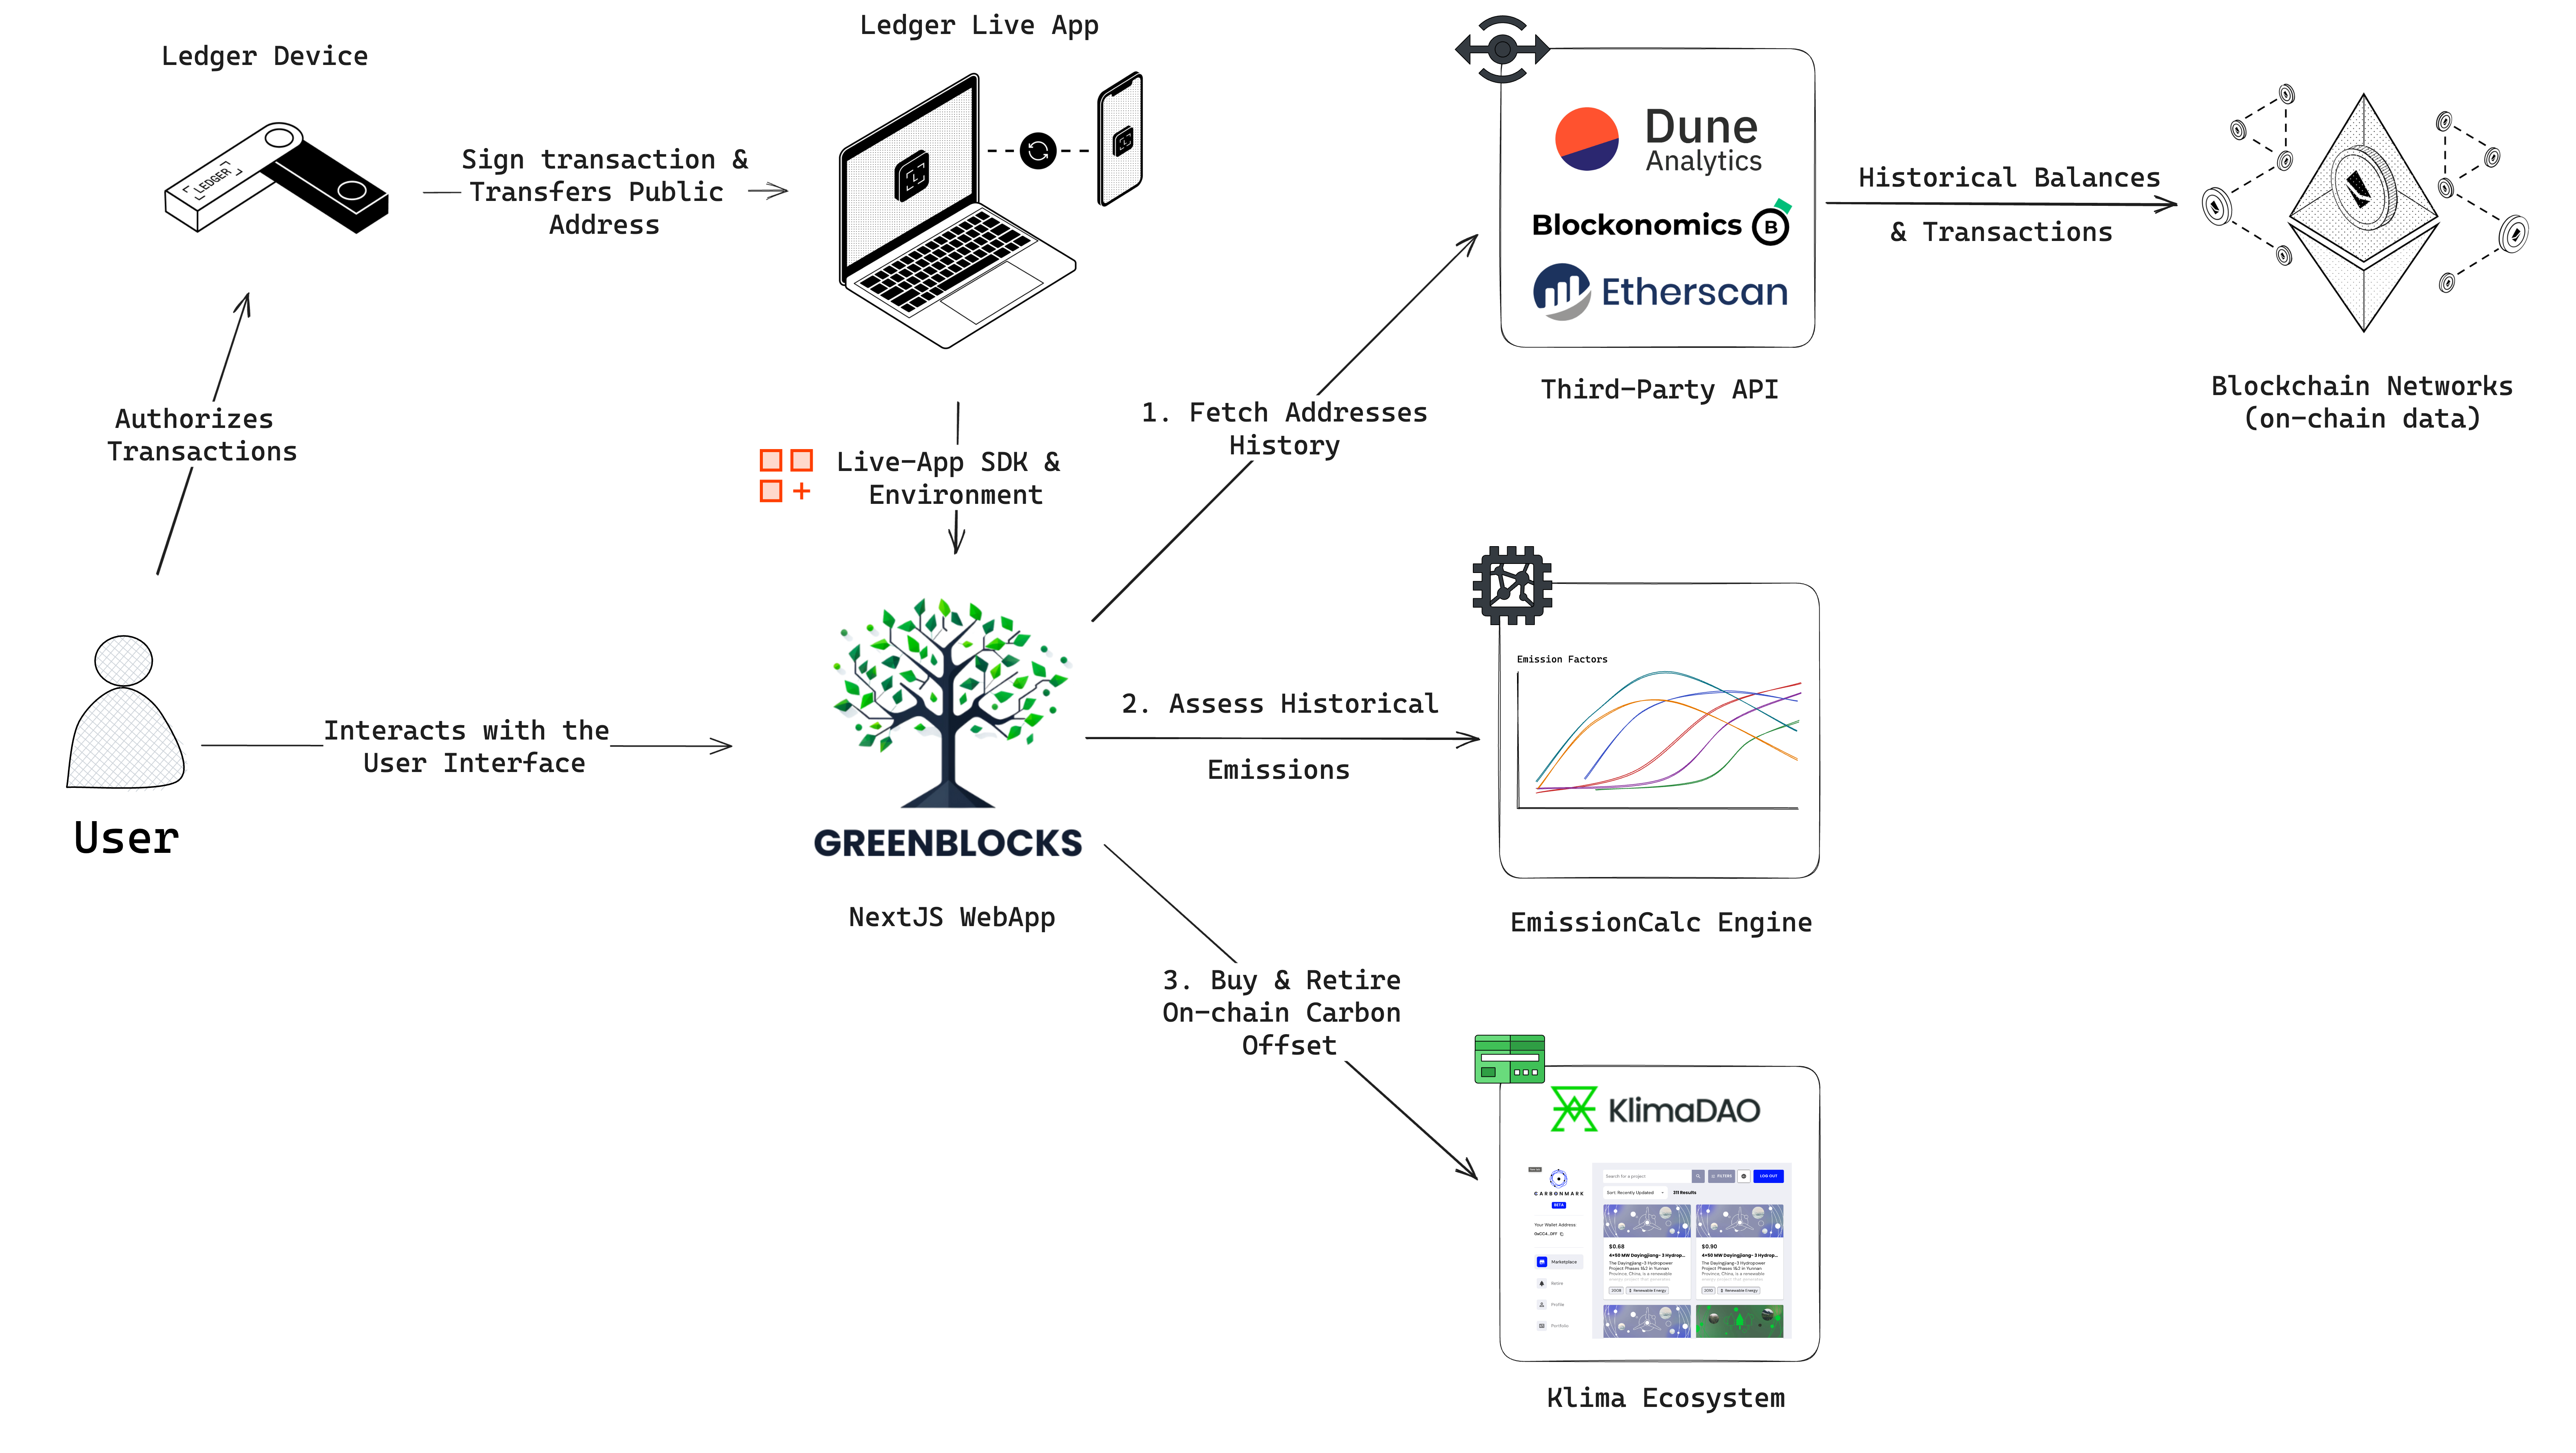
\includegraphics[scale=0.08]{figures/functionnal architecture.png}}
    \caption{GreenBlocks - Functionnal Architecture}
    \label{fig:functionnal_architecture}
\end{figure}

\begin{figure}[hbt!]
    \centering
    \centerline{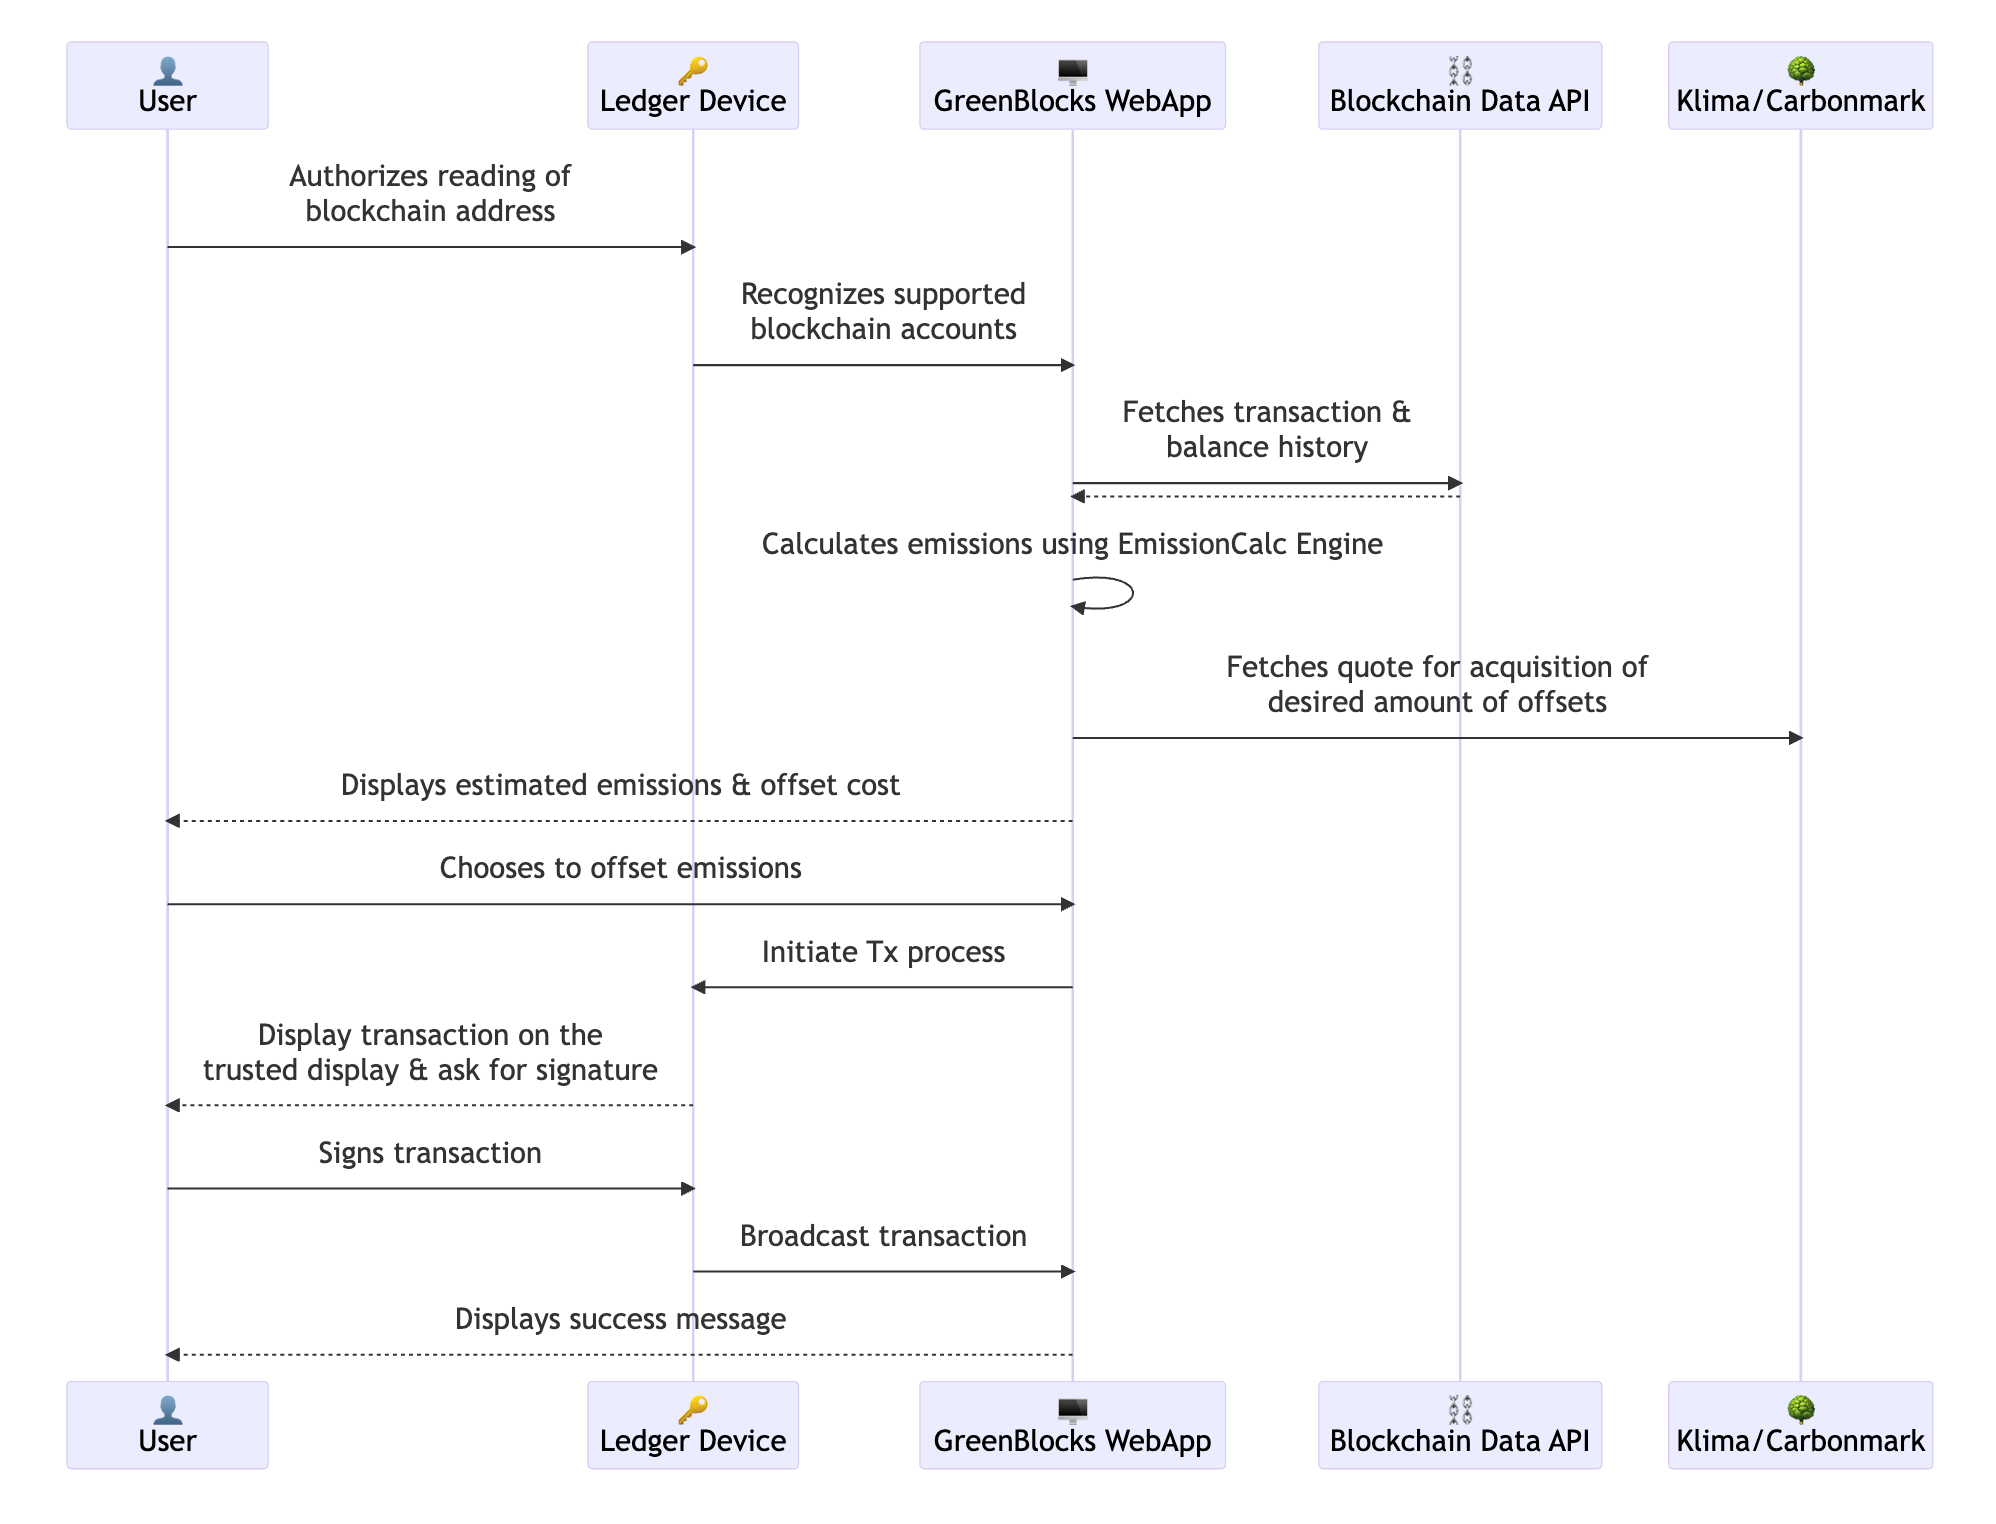
\includegraphics[scale=.27]{figures/sequence.png}}
    \caption{GreenBlocks - Sequence Diagram}
    \label{fig:sequence}
\end{figure}

\change{Review figure size for readability. Consider redo on lucid to control font}


\section{System Architecture and Components}
\subsection{User Interface Layer}
\subsection{Middleware Layer}
\subsection{Backend Layer}
\subsection{Data Layer}
\section{Development Process}

\chapter{Discussion}
\section{Results and Analysis}
\section{Comparative Analysis: Different User Profiles and Protocols}
\begin{enumerate}
    \item Bitcoin holder
    \item Bitcoin trader
    \item Ethereum holder
    \item Ethereum App user
    \item Ethereum only since merge (or show all using a time-series on emissions)
\end{enumerate}

\section{Statistical Analysis}
\todo{Statistical analysis of a random sample of addresses}
\unsure{will it be possible to get a sample of bitcoin xpub. Otherwise focus on ethereum analaysis before \& post merge}

\subsection{Validation and Sensitivity Analysis Results}
\subsubsection{Validation Results}
\subsubsection{Sensitivity Analysis Findings}

\section{Limitations and Future Work} \label{se:limitations}
\section{Further Opportunities for Blockchain and Sustainability}

\chapter{Conclusion}


\bibliography{bibliography.bib}


\end{document}